%%%% ijcai11.tex

\typeout{IJCAI-11 Instructions for Authors}

% These are the instructions for authors for IJCAI-11.
% They are the same as the ones for IJCAI-07 with superficical wording
%   changes only.

\documentclass{article}
% The file ijcai11.sty is the style file for IJCAI-11 (same as ijcai07.sty).
\usepackage{ijcai11}

% Use the postscript times font!
\usepackage{times}

\usepackage[utf8]{inputenc}
\usepackage[catalan]{babel}

\usepackage{graphicx}

% the following package is optional:
%\usepackage{latexsym} 

% Following comment is from ijcai97-submit.tex:
% The preparation of these files was supported by Schlumberger Palo Alto
% Research, AT\&T Bell Laboratories, and Morgan Kaufmann Publishers.
% Shirley Jowell, of Morgan Kaufmann Publishers, and Peter F.
% Patel-Schneider, of AT\&T Bell Laboratories collaborated on their
% preparation.

% These instructions can be modified and used in other conferences as long
% as credit to the authors and supporting agencies is retained, this notice
% is not changed, and further modification or reuse is not restricted.
% Neither Shirley Jowell nor Peter F. Patel-Schneider can be listed as
% contacts for providing assistance without their prior permission.

% To use for other conferences, change references to files and the
% conference appropriate and use other authors, contacts, publishers, and
% organizations.
% Also change the deadline and address for returning papers and the length and
% page charge instructions.
% Put where the files are available in the appropriate places.

\title{Implementació de la teoria de resta de\\formes desenvolupada en el grup C4R2}
\author{Ivan Barrachina Bellmunt i Josep López Centelles\\
II-80 Intel·ligència Artificial avançada\\
Universitat Jaume I Castelló\\
Avda. Vicent Sos Baynat s/n, 12071 Espanya \\
al106647@uji.es, al106650@uji.es}

\begin{document}

\maketitle

\begin{abstract}
Aquest article explica el treball realitzat per a implementar la teoria de resta de formes definida pel grup C4R2 [Mus09].
Com a objectiu final s'ha obtingut una interfície gràfica que ens permet elegir dos figures, de les quals es calcula la resta, i es mostra tant el resultat com la seua descripció qualitativa.
\end{abstract}

\section{Introducció}
El treball que es planteja a continuació tracta de presentar la teoria de la resta de formes i la integració d'aquesta en una interfície gràfica.
Existeixen algunes limitacions que no permeten fer qualsevol resta de formes però s'ha intentat que aquesta versió del software accepte la majoria d'elles.
\\
\\
La intel·ligència artificial és considerada una rama de la computació i relaciona un fenomen natural amb una analogia artificial a través de programes de computador.
De manera més específica la intel·ligència artificial és la disciplina que s'encarrega de construir processos que al ser executats sobre una arquitectura física produeixen accions o resultats que maximitzen una mesura de rendiment determinada, basant-se en la seqüència de entrades percebudes i el coneixement emmagatzemat en dita arquitectura.
\\
\\
Aquest projecte es centra en la interpretació de les característiques qualitatives per a definir la nova figura.
L'analisis de característiques qualitatives és una de les facultats que té la ment humana i s'utilitza a diari.
Implementant aquest procés dotem al nostre software d'una intel·ligencia artificial clara, ja que es simula una forma de pensar molt humana.
\\
\\
\subsection{Aquest treball dintre de la intel·ligencia artificial}
El treball que anem a desenvolupar tracta sobre l'obtenció d'imatges, anàlisis de les seves característiques i finalment la realització d'una operació en la que s'utilitzen dos figures per obtindre el resultat de la seva resta.
Açò pot ser utilitzat posteriorment per a definir mosaics d'una forma intel·ligent i amb la seguretat d'evitar errors.
La primera part del projecte que consta de l'obtenció dels vèrtex d'una figura correspon al camp de la visió, mentre que l'anàlisi i els seus resultats pertanyen al camp del raonament qualitatiu, dins de la intel·ligència artificial.
\\
\section{Descripció qualitativa de les figures}
Com s'ha dit anteriorment, en aquest treball s'utilitzarà la descripció qualitativa de figures, obtinguda mitjançant l'executable desenvolupat en [Mus07].
La descripció qualitativa consisteix en l'assignació de valors de les principals característiques de cada vertex de la figura dins de rangs definits qualitativament.
En aquests rangs no hi ha valors enterns sino conceptes que determinen en quin rang es trova cadascuna dels valors reals.
Per exemple, un angle no es determina mitjançant el nombre de graus que conté sino que es descriurà definint el seu rang: molt agut, agut, recte, obert, molt obert.
\\
\\
Les característiques que determinen cada vertex són el tipus d'angle, la seua convexitat i la llargària de les seues arestes respecte les seues veïnes.
Per a poder exlicar com es realitzen els cálculs de la descripció qualitativa usarem els tres vertexs participants en cada càlcul.
Anomenarem aquest punts com i(anterior), j(vertex que s'està calculant) i k(següent) per a facilitar l'explicació dels càlculs.
\\
\subsection{Tipus d'angle}
Per classificar l'angle del vèrtex j, dibuixarem un cercle amb diàmetre i k, que és la línia d'unió entre els vèrtexs i (anterior) i k (següent).
Si el vèrtex que estudiem es troba a l'interior del cercle, l'anomenarem obtús (obtuse), si es troba en l'exterior l’anomenarem agut (acute) i si coincideix en la circumferència serà recte (right-angle).
\\
\\
A més, si els angles són molt aguts (0-40 graus) o molt obtusos (140-180 graus) es defineixen com very obtuse o very acute.
Es pot observar en la Figura~\ref{fig:angulos} com es defineix alguns tipus d'angles.
\\

\begin{figure}[h]
\centering
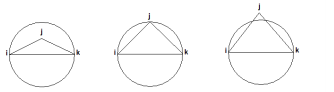
\includegraphics[width=260pt]{images/angles.png}
\caption {Exemples de l'estudi de la classificació de tres angles, un obtús, un recte i un tercer agut.}
\label {fig:angulos}
\end{figure}

\subsection{Convexitat}
Per calcular el tipus de convexitat de l’angle del vèrtex j, realitzem una línia del vèrtex anterior al posterior.
Si aquest vèrtex j es troba a l'esquerra d'aquesta línia, direm que l'angle és convex i si es troba a la dreta, còncau.
En la Figura~\ref{fig:convex} s'observen els dos posibles exemples de les diferents convexitats.

\begin{figure}[h]
\centering
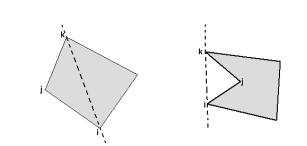
\includegraphics[width=260pt]{images/convex.jpeg}
\caption {Exemple de la convexitat de dos angles, un primer convex i un còncau.}
\label {fig:convex}
\end{figure}

\subsection{Llargària de les arestes}
Per calcular la llargària de les arestes del vèrtex  j, compararem la distància euclídea de les línies i-j i j-k.
\\
\\
D(j-k)=)=((Xk-Xj)2+(Yk-Ykj)2)1/2
\\
\\
D(i-j)=)=((Xj-Xi)2+(Yj-Yki)2)1/2
\\
\\
Comparant aquestes dos dades obtenim el valor de la llargària de les arestes:
\begin{itemize}
\item Si D(j-k) = [0, 0,4]   D(i-k) $\rightarrow$  Molt menor (much-shorter)
\item Si D(j-k) = [0.4, 0.6] D(i-k) $\rightarrow$  Mitad (half-lenght)
\item Si D(j-k) = [0.6, 0.9] D(i-k) $\rightarrow$  Un poc menor (a-bit-shorter)
\item Si D(j-k) = [0.9, 1.1] D(i-k) $\rightarrow$  Igual (similar-lenght)
\item Si D(j-k) = [1.1, 1.9] D(i-k) $\rightarrow$  Un poc major (a-bit-longer)
\item Si D(j-k) = [1.9, 2.1] D(i-k) $\rightarrow$  Doble (double-lenght)
\item Si D(j-k) = [2.1, n]   D(i-k) $\rightarrow$  Molt major (much-longer)
\end{itemize}

\subsection{Connexió}
És el tipus d'aresta connectada i pot ser: line-line(ll), line-curve (lc), curve-curve(cc), curve-line (cl) o curvature-point (cp). En el nostre cas al restar figures poligonals sempre serà ll ja que no hem tractat el problema de restar figures amb arestes que no siguen rectes.
\\
\\
\subsection{Descripció completa de la figura}
Ja explicades totes les característiques de cada vertex, sols necessitem definir un estandard per a mostrar tota la informació.
Iniciant desde el primer vertex (el que estiga més amunt i a l'esquerra) es va mostrant tota la informació de tots els vertexs com es pot veure en aquest exemple:
  
\begin{center}
\emph{[Con1,Cur1,Lon1,Conv1]...[ConN,CurN,LonN,ConvN]}
\end{center}

Aquest exemple respon a la descripció de vertex explicada en la teoria de Zoe[Biblio..], segons la qual els vèrtex d'una figura es descriuen com una tupla $<$ Con; Cur; Lon; Conv $>$ on:

\begin{itemize}
\item \emph{Con} és el tipus d'aresta conectada.
\item \emph{Cur} és la curvatura, l'angle del vèrtex.
\item \emph{Lon} és la longitud comparada de l'aresta anterior respecte a la següent.
\item \emph{Conv} és la convexitat del vèrtex.
\end{itemize}

Els valors de cadascuna de les anteriors característiques s'han definit anteriorment de forma que la descripció d'una figura quedaria com el següent exemple:
\\
\\
TODO: ficar el exemple

\subsection{Limitacions de les figures}
Quan es realitza una operació de diferència, existeix un minuend al que se li resta un substrahend per obtindre un resultat, la diferència. En el cas de restar figures, existeixe una sèrie de restriccions que aquetestes deuen cumplir per a que els càlculs funcionen correctament.

La diferència es realitzarà sempre per el primer vèrtex de la descripció de la figura minuend. Açò vol dir, per el vèrtex amb menor y i menor x (les x del plà van de esquerra a dreta i les y de amunt a aball).

El minuend sempre deu ser major que el substrahend, En el cas de les figures, per a comprovar que aquesta restricció es cumpleix, es deuen comprovar que ningun dels punts característics del substrahend es surt de la frontera del minuend.

-En el cas de tindre varies peces com posible substrahend, haurem d’elegir una, seguint els següents criteris:

    -Que tinga un angle que siga el mes semblant possible a l’angle per el que es realitza la diferència. Açò és:

        1. Que siga el mateix tipus d’angle.

        2. Que la longitud de les dos arestes siga el més semblant possible a les del minuend.

-En cas que no existeixca ninguna peça amb el mateix tipus d’angle, s’escollirà un amb un angle amb el següent rang més menut, però el mes similar possible. Açò és, si el angle del minuend es r i no hi ha substrahends amb angle r, elegir una peça amb angle a.

-Si existeixen varies figures que complisquen les caracterśitiques, s’escollis la que tinga major àrea, de forma que quede menys zona a emplenar.


%% The file named.bst is a bibliography style file for BibTeX 0.99c
\bibliographystyle{named}
\bibliography{ijcai11}

\end{document}

